\documentclass[times, utf8, diplomski]{fer}
\usepackage{booktabs}
\usepackage{fixltx2e}
\usepackage[options]{mcode}
\begin{document}

% TODO: Navedite broj rada.
\thesisnumber{1233}

% TODO: Navedite naslov rada.
\title{Obrada i analiza govora na ugradbenom računalnom sustavu u stvarnom vremenu}

% TODO: Navedite vaše ime i prezime.
\author{Paula Franić}

\maketitle

% Ispis stranice s napomenom o umetanju izvornika rada. Uklonite naredbu \izvornik ako želite izbaciti tu stranicu.
\izvornik

% Dodavanje zahvale ili prazne stranice. Ako ne želite dodati zahvalu, naredbu ostavite radi prazne stranice.
\zahvala{}

\tableofcontents
\listoffigures
\chapter{Uvod}
Digitalna obrada signala (DSP) svoj početak zabilježila je razvojem prvih digitalnih računala 60-ih i 70-ih godina prošlog stoljeća. Naravno, takva računala su bila izrazito skupa tako da se i primjena obrade signala koristila isključivo u vojne svrhe, medicini te razvoju radara i sonara, točnije u svrhe koje su ovisile o velikim financijskim ulaganjima.

Napretkom razvoja digitalnih računala, DSP je svoje uporište našao u razvoju komercijalnih proizvoda kakve danas poznajemo. Tako smo danas upoznati s digitalnim uređajima za obradu zvuka, slike, videa i slično.

Prije daljnje rasprave o digitalnoj obradi signala, razjasnit će se zašto se ona smatra posebnim područjem u inženjerstvu jest što obrađuje jedinstvenu vrstu podataka: signale. Signali su podatak koji najčešće dolazi iz prirode. Tako se njihovom obradom pokušava manipulirati kako bi se postigli ciljevi poput: poboljšanja kvalitete slike, kvalitete zvuka, videa, izdvajanje određenih značajki signala za potrebe raspoznavanja te kompresija.

U ovom radu fokusirat ćemo se na digitalnu obradu zvuka, točnije govora. Zvuk je longitudinalni val koji se vibracijama širi po prostoru, organ koji ga percipira jest uho. 

Tako ćemo kroz rad proći osnovni dio vezan uz anatomiju uha kako bismo mogli razjasniti koncept uređaja koji akvizira zvuk te ga obrađuje, specifikacije potrebnih komponenti za akviziciju i obradu zvuka (mikrofon, A/D pretvornik, mikrokontroler) te će fokus biti na implementaciji dogotalne obrade govora na ugradbenom računalnom sustavu u stvarnom vremenu.

\chapter{Analiza govora}
\section{Nastanak glasa}
Glas nastaje izbacivanjem zraka iz pluća koji putem grkljana, dolazi do glasnica. Prolaskom zraka kroz glasnice one vibriraju pa na taj način nastaje glas. Nakon prolaska glasa kroz glasnice, ono ulazi u ždrijelo te u usnu i nosnu šupljiu gdje se ton glasa mijenja te oblikuje. U oblikovanju glasova sudjeluje jezik, zubi, usne, nepce i čeljust.
Kod oblikovanja nastalog glasa, bitno je poznavati funkciju vokalnog trakta. Vokalni trakt se u širem smislu sastoji od sljedećih osnovnih dijelova:
\begin{itemize}
\item prostor izmedu glasnica, glottis
\item pharynx ili ždrijelo (veza usta i jednjaka)
\item usna šupljina
\item jezik
\item stražnje (meko) nepce
\item srednje nepce
\item prednje (tvrdo) nepce
\item nadzubno meso
\item zubi
\item usne
\item velum ili resica zatvara usnu šupljinu prema nosnoj
\item nosna šupljina koja završava s nosnicama
\end{itemize}
Vokalni trakt se ponaša kao svojevrstan filtar, koji će spektralno obojiti pobudni signal. Slično kao što se geometrijom cijevi kod orgulja određuje ton (visina i spektralni sastav) signala koji se formira, tako ce i geometrijski oblik vokalnog trakta određivati koje se spektralne komponente signala pojačavaju, a koje prigušuju.


\begin{figure}[hbt!]
 \centering
 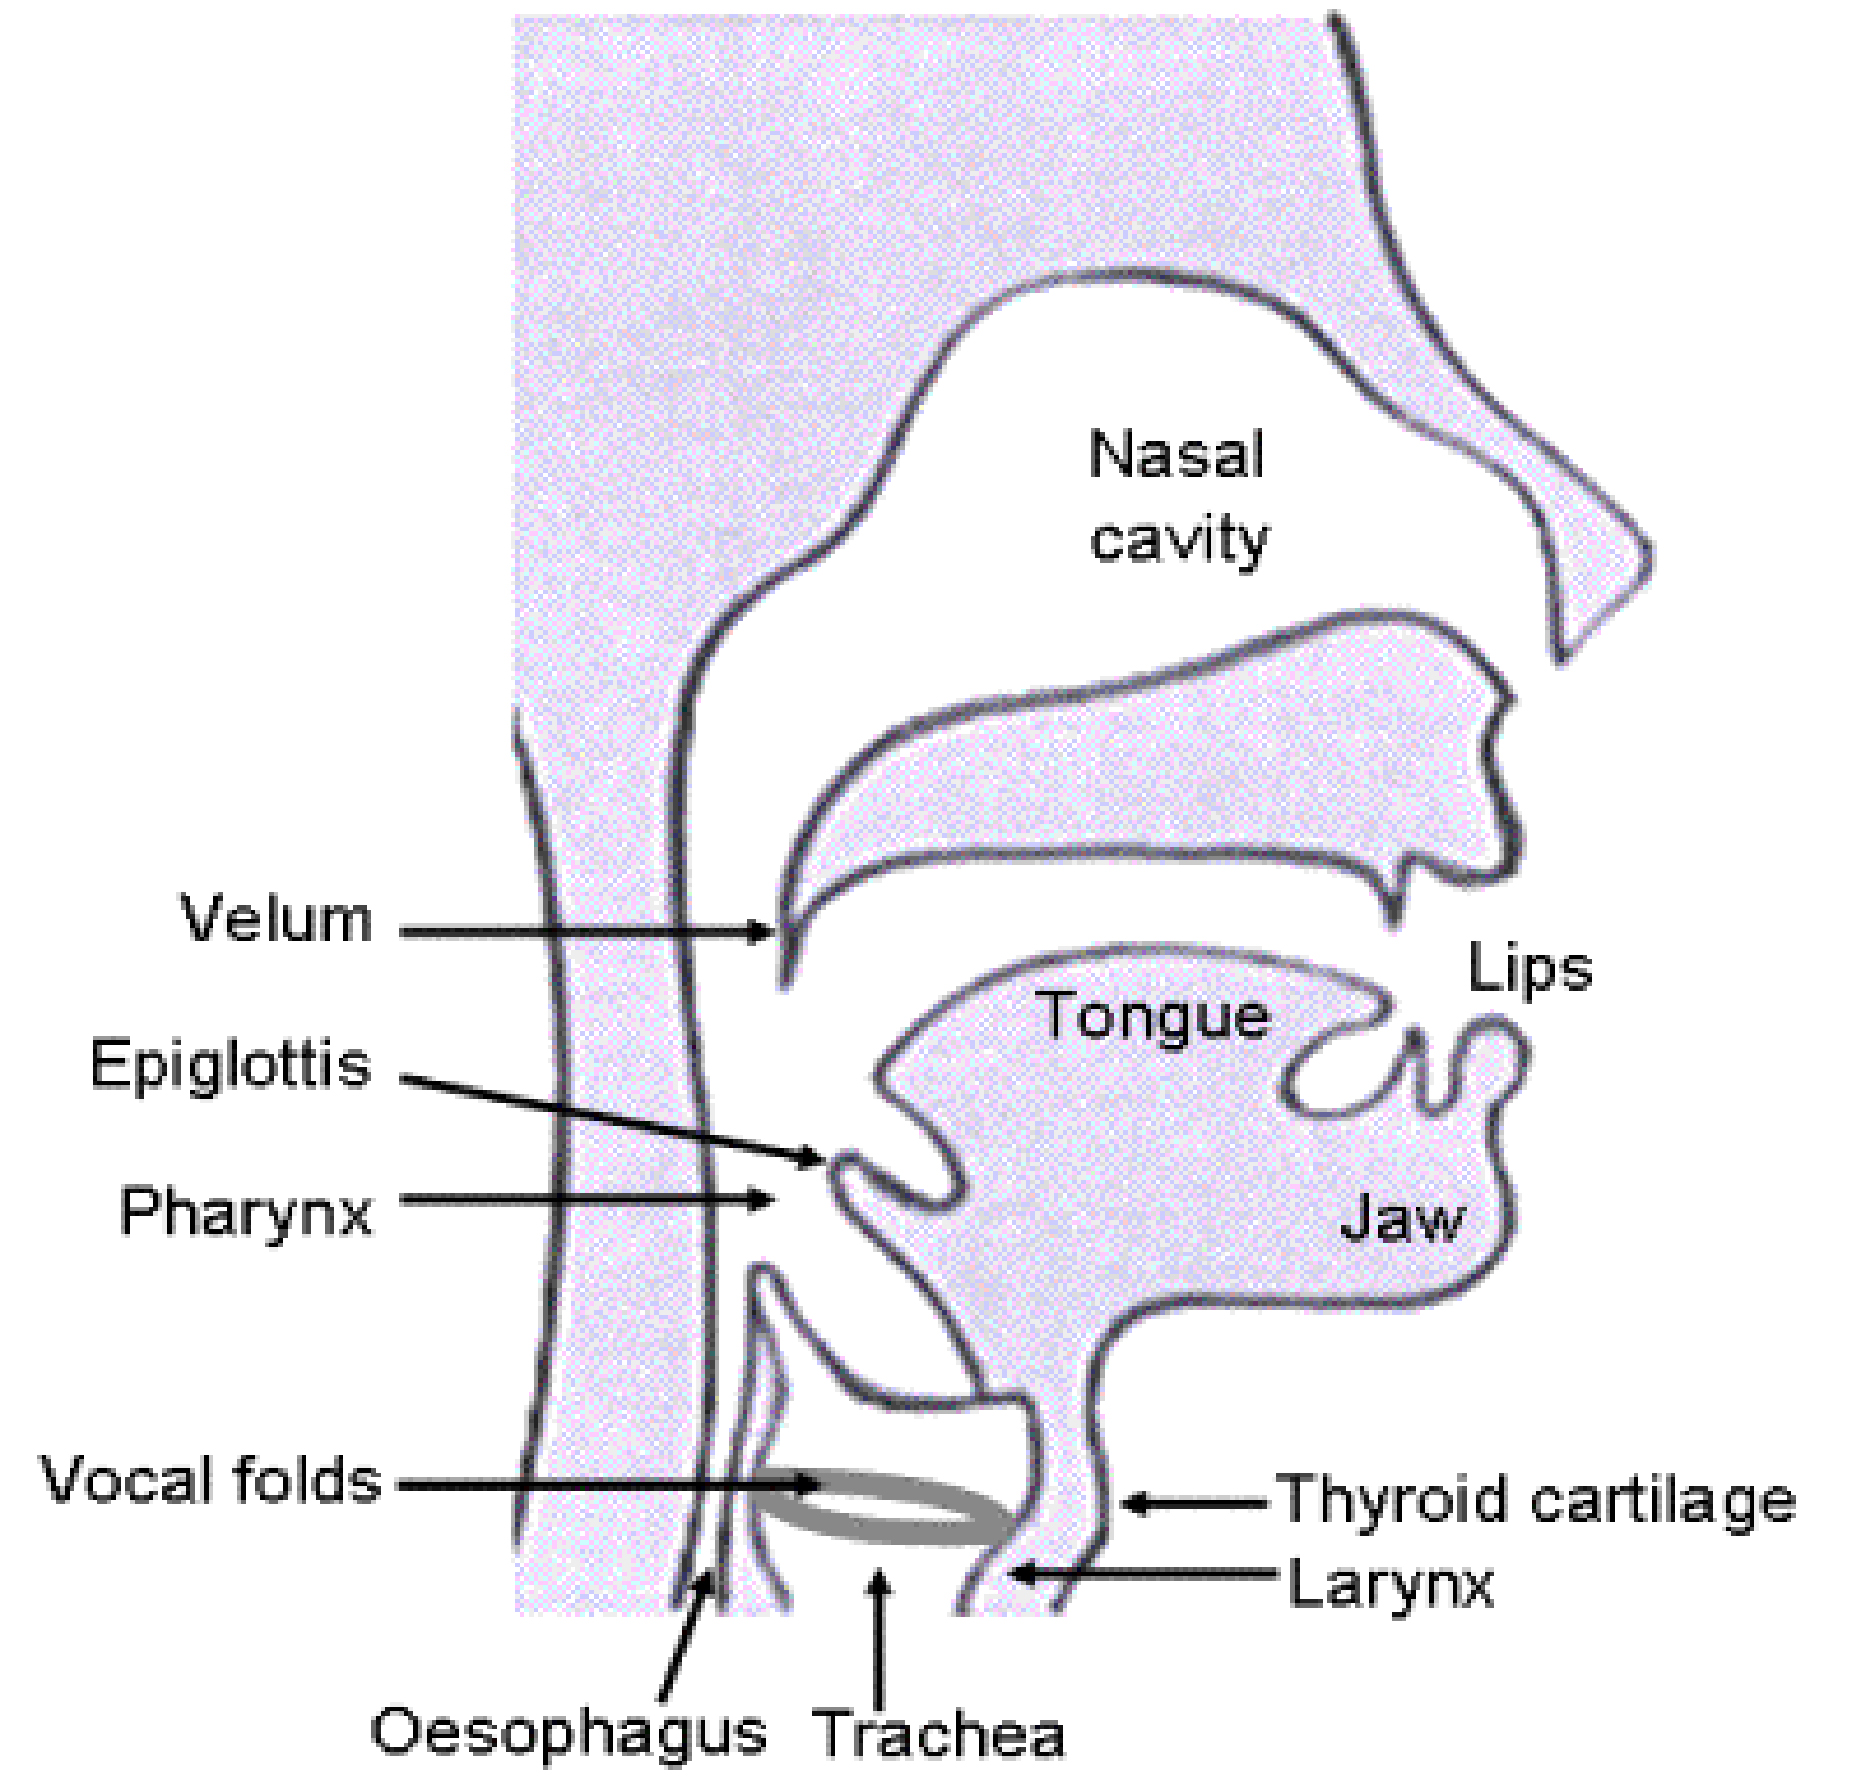
\includegraphics[scale=0.5]{photos/vokalni trakt.jpg}
 \caption{Anatomija ljudskog vokalnog trakta}
 \label{trakt}
\end{figure}

\section{Karakteristike glasa}
Ljudski glas je jedini koji može istovremeno proizvesti riječ i ton. Osnovne karakteristike glasa su: visina, intenzitet i boja. Dotaknut ćemo se i formanata jer njihovo postojanje uvelike utječe na frekvencijsku karakteristiku vokalnog trakta. 

\subsection{Visina glasa}
Visina glasa (ton) je perceptivni fenomen, a ovisi o fundamentalnoj frekvenciji koja je fizikalni parametar. Fundamentalna frekvencija (u daljnjem tekstu $F_{0}$) je broj vibracija koje glasnice proizvedu u jednoj sekundi. Što je veći broj vibracija glasnica, viša je vrijednost fundamentalne frekvencije pa i glas doživljavamo višim. Brzina titranja glasnica ovisi o debljini, dužini i napetosti glasnica, te o tlaku zraka koji prolazi između glasnica. Povišenje tlaka zraka dovodi istovremeno do povećanja intenziteta glasa i višeg tona. Na vrijednost $F_{0}$ utječu dob, spol, tjelesna konstitucija, socijalno okruženje, emocije, intelektualni status. Prosječna $F_{0}$ muškog glasa iznosi oko 120 Hz, a ženskog 225 Hz. Istraživanja $F_{0}$ djece još su složenija zbog čimbenika rasta i razvoja pa su podaci nekompletni, no zna se da je $F_{0}$ prvog plača vrlo visoka i kreće se između 400 i 600 Hz. Porastom kronološke dobi djeteta $F_{0}$ pada. Tako npr. za dječake kronološke dobi 10,5 godina vrijednost $F_{0}$ iznosi oko 250 Hz.

\subsection{Intenzitet}
Intenzitet ili jakost glasa percipiramo kao glasnoću, a ovisi o amplitudi titranja glasnica, te o  subglotičkom tlaku zraka\footnote{Zračni tlak u plućnim alveolama}. Što su te vrijednosti više, veća je i jačina glasa. Intenzitet se izražava u decibelima (dB). Intenzitetski raspon od tek čujnog glasa do najglasnijeg koji pojedinac može izvesti iznosi i do 70 dB. Ovu razliku između pianissima i fortissima, tj. najmanje i najveće razine zvuka nekog izvora, nazivamo dinamikom.

\subsection{Boja glasa}
Boja glasa je karakteristika glasa koja čini glas prepoznatljivim za određenog sugovornika. To je perceptivni fenomen koji svaki glas čini jedinstvenim i neponovljivim. Nastaje kao rezultat rezonancije, tj. obrade, ili možda bolje, dorade zvuka na putu od glasnica do izgovora. Taj put je vokalni trakt, a čine ga rezonantne šupljine, ili kraće, rezonatori. Boja glasa ima stalnu i promjenjivu sastavnicu. Stalna ovisi o  nasljednim i stečenim anatomsko-fiziološkim karakteristikama, ali isto tako i o načinu uporabe organa za glasanje na što utječe i kulturno okruženje. Promjenjiva sastavnica boje glasa odnosi se na izražajnu mogućnost govornika. Nadalje, o boji glasa prosuđuje se s biološkog, psihološkog, kulturnog, estetskog i patološkog stajališta što potvrduje koliko je ova karakteristika glasa složena, a opisi i definicije katkad i vrlo različiti. Sinonim za boju glasa je timbar, a u angloameričkoj literaturi vokalna kvaliteta ili kvaliteta glasa što je, zapravo, i širi pojam. U tom kontekstu, glas se opisuje kao pun, voluminozan, kreštav, dahtav, nazalan, drhtav, napet, šuškav, pucketav, zvonak, taman, promukao i slično \citep{optimala}. 

\subsection{Formanti}
Ono što će nam također utjecati na frekvencijski spektar glasa je duljina vokalnog trakta (prije spomenuti faktor kod nastajanja glasa) te veličina otvora na glotisu i ustima. Tu je bitno upoznati se s formantima. Formanti su intenzitetski naglašeni dijelovi spektra nastali rezoniranjem šupljine izgovorom nekog glasa. Možemo uočiti što je veći odnos presjeka otvora i duljine vokalnog trakta to je formant viši. Obično kod analize glasova primjećujemo tri formanta. Drugi formant je viši u smislu što se suženje pomiče prema ustima te što je veći odnos presjeka i duljine vokalnog trakta.

Sve ove karakteristike određuju frekvencijski spektar glasa. Znamo da ljudsko uho čuje 20 Hz do 20 kHz. Niže frekvencije nose informacije o govoru, dok visoke frekvencije doprinose jasnoći govora. Vidimo na slici \ref{raspon} podjelu područja na tri glavne cjeline, niske, srednje i visoke frekvencije. Ova informacija je bitna kod spektralne analize glasova.

\begin{figure}[hbt!]
 \centering
 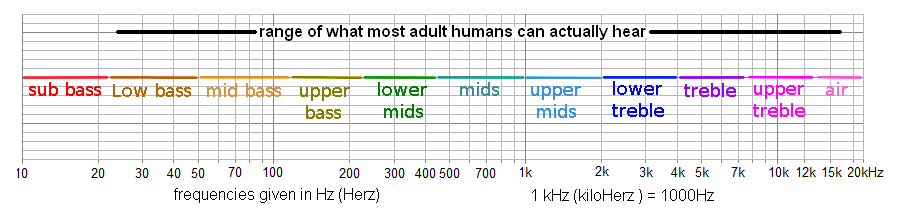
\includegraphics[scale=0.5]{photos/raspon.png}
 \caption{Raspon frekvencija audio frekvencija koje spadaju pod ljudsko slušno područje}
 \label{raspon}
\end{figure}


\chapter{Analiza sluha}
\label{chap:sluh}
Nakon pojašnjenja nastanka te karakteristika govora, potrebno je objasniti rad organa za sluh i slušanje: uho.

Akvizicija zvuka počinje s vanjskim uhom. Kada je zvuk putuje prema vanjsko uhu, zvučni valovi, ili vibracije, putuju niz vanjski slušni kanal i udaraju u opnu (bubnjić). Bubnjić vibrira te se te vibracije zatim prenose na 3 sićušne kosti u srednjem uhu koje se nazivaju koščice (čekić, nakovanj i stremen). Koščice se ponašaju kao pojačalo zvuka. One zatim šalju zvučne valove u unutarnje uho i u slušni organ ispunjen tekućinom (pužnica).

\begin{figure}[hbt!]
 \centering
 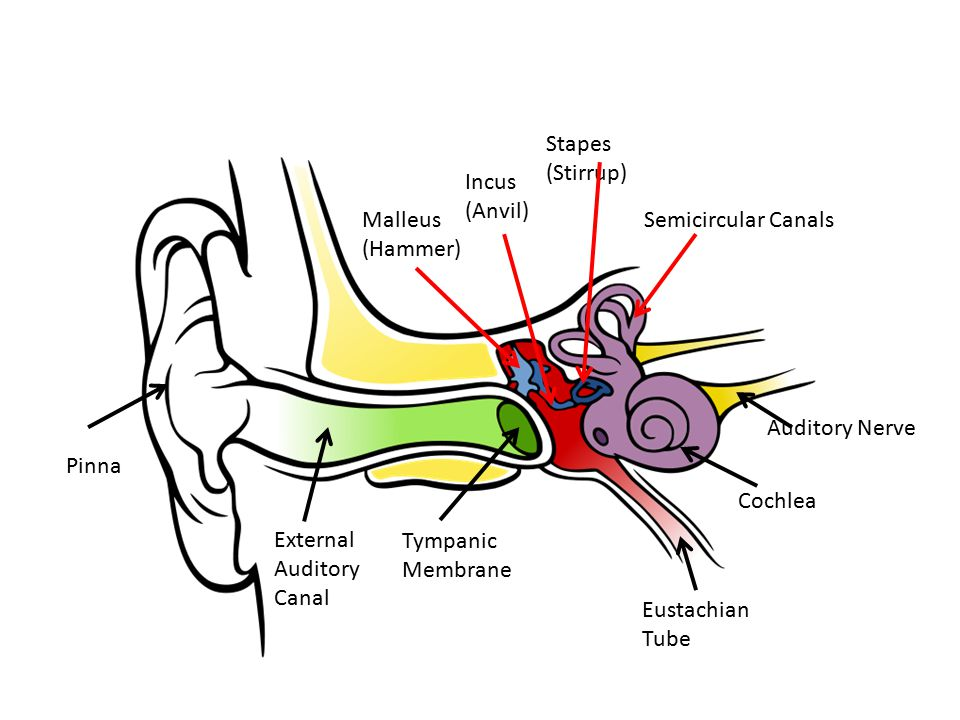
\includegraphics[scale=0.5]{photos/earanatomy.png}
 \caption{Anatomija uha }
\end{figure}

Kada zvučni valovi dosegnu unutarnje uho, oni se pretvaraju u električne impulse. Slušni živac šalje ove impulse u mozak. Mozak tada prevodi ove električne impulse kao zvuk\citep{uho}.

Jedna od bitnijih značajki uha jest što je ono, uz osjetilo vida, jedino osjetilo koje jačinu signala percipira po logaritamskoj skali. Znamo također da razlike u jačini snage između najtišeg i najglasnijeg zvuka koje ljudsko uho može percipirati jest $10^6$.

Također, prilikom obrade zvuka, moramo na umu imati da čovjek ima dva uha, tako da vrši akviziciju iz dva smjera te tako može percipirati smjer dolaska zvuka. Ovo nam je također bitno kod obrade kako bi imali dva izlaza koji simuliraju stereo zvuk.

Zanimljiva karakteristika uha jest ovisnost frekvencijskog odziva prema glasnoći zvuka, što možemo vidjeti na slici \ref{flemu}. Tu možemo uočiti nejednaku osjetljivost uha na niske frekvencije

\begin{figure}[hbt!]
 \centering
 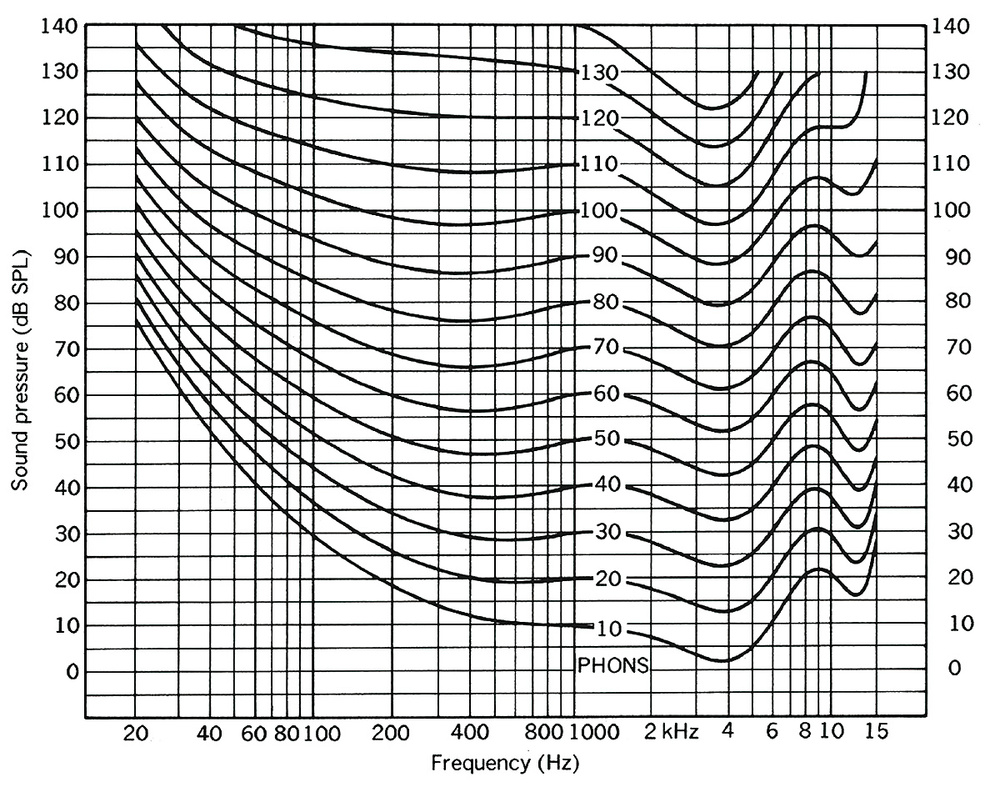
\includegraphics[scale=0.4]{photos/flemu.jpg}
 \caption{Fletcher-Munson krivulje}
 \label{flemu}
\end{figure}
Govor spada pod već spomenute zvučne signale. Kao što je u poglavlju \ref{chap:sluh} objašnjeno, ljudsko uho može percipirati signale frekvencija od 20 Hz do 20000 Hz. Ljudski govor spada u područje od 200 Hz do 5000 Hz, ovisno o spolu i dobi osobe. Iako je tu već očigledno da nam neće biti potreban spektar iznad 5000 Hz, nastojat ćemo ga zadržati nakon očitavanja kako ne bi gubili na kvaliteti signala, što nam je u ove svrhe bitno.

\chapter{Sustav za obradu i analizu govora}
Za razvoj sustava čija je svrha obrada i analiza govora koristi se MATLAB za generiranje filtarskih realizacija za obradu govora te STM32F4-Discovery ugradbeni sustav kojim će se vršiti akvizicija i filtracija signala. Napravit će se pregled već dostupnih tehnologija za obradbu audio signala (u našem slučaju govora).




\section{STM32F4-Discovery}

\subsection{Glavne značajke ugradbenog računalnog sustava}
Sustav koji želimo razviti za potrebe obrade govornog signala nam zahtjeva ključne komponente:

\begin{enumerate}
\item procesor sa DSP značajkama
\item analogno-digitalni pretvornik s performansama prilagođenim za audio signale
\item MEMS mikrofon koji vrši akviziciju signala
\end{enumerate}

Kod ovakvog sustava potrebno je pobrinuti se da je akvizicija signala brza i ne narušava inicijalnu frekvencijsku karakteristiku glasa te da je obrad signala brza i kvalitetna. 

Naš ugradbeni računalni sustav jest STM32F407VG. On sadrži ARM Cortex-M4 procesor sa DSP značajkama koji će nam biti ključan za daljnju obradu signala. Ovaj mikrokontroler već ima ugrađeni MEMS mikrofon i A/D pretvornik no oni su namijenjeni za opću primjenu, dok su nama potrebne komponente za isključivu obradu audio signala tako da će se u daljnjim potpoglavljima napraviti usporedba dostupnih te traženih komponenti.

\section{DSP Procesor}
\label{instr}
Odabrani ugradbeni računalni sustav sadrži ARM-ov procesor Cortex-M4. Ovaj procesor spada u familiju Cortex-M procesora koji se koriste za ovakve svrhe. Glavne karakteristike takvih procesora je visoka efikasnost potrošnje energije, mala površina procesora, kratki cjevovodi te rad na frekvenciji oko 200 MHz \citep{cortexm4}.

Ono što čini ovaj procesor pogodnim za digitalnu obradu audio signala jest što ima podršku za funkcije tog tipa pomoću SIMD i MAC instrukcija.

\textit{Single Instruction Multiple Data} (SIMD) je skupina instrukcija koje omogućuju paralelno izvođenje operacije za više podataka.

\begin{figure}[hbt!]
 \centering
 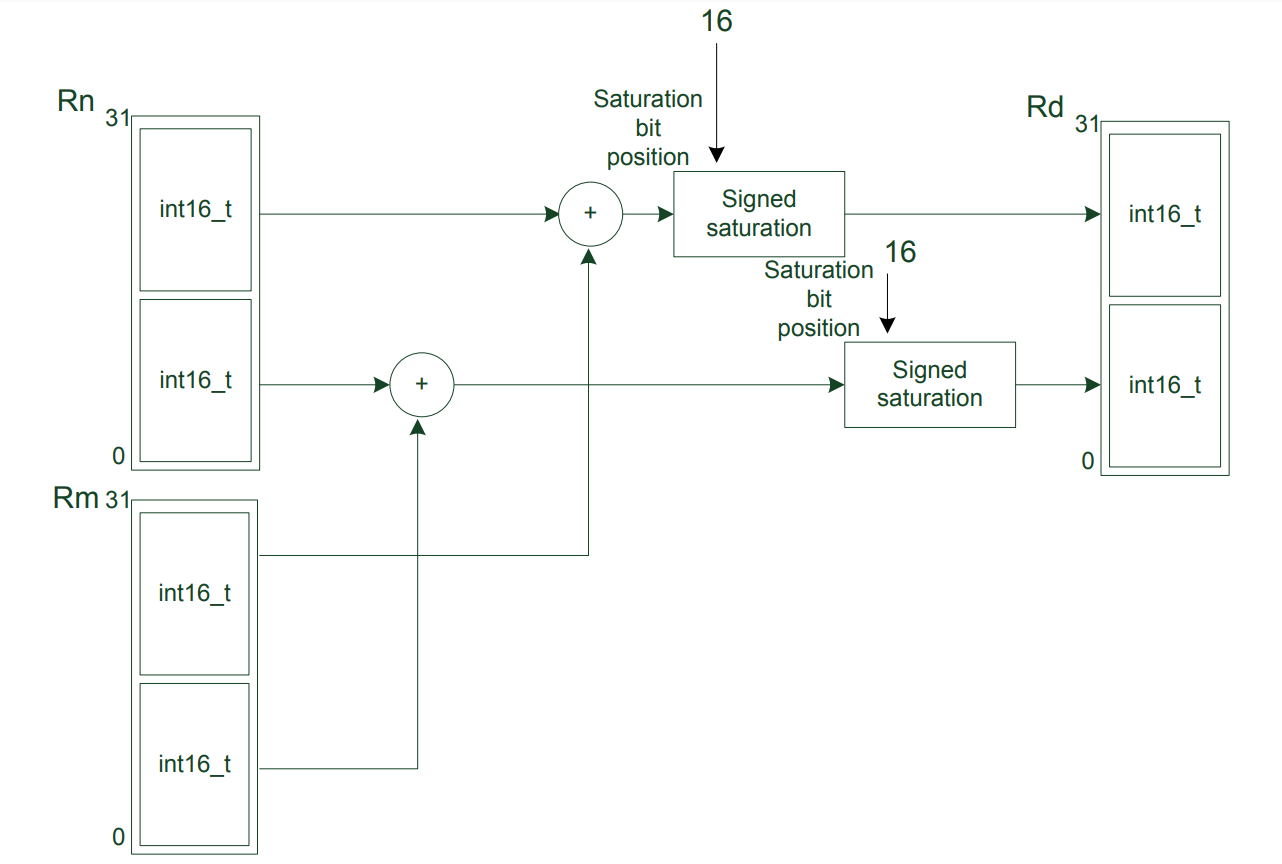
\includegraphics[scale=0.4]{photos/simd.png}
 \caption{Dijagram izvođenja SIMD instrukcije zbrajanja}
 \label{SIMD}
\end{figure}

Kao što se vidi na slici \ref{SIMD}, podatke koje želimo zbrojiti podijelimo na nižih 16 bita i viših 16 bita. Kod oba podatka zbrajaju se posebno niži bitovi i posebno viši bitovi. Ono što je ključno kod SIMD naredbe jest aritmetika zasićenja. U slučaju da zbroj nižih ili viših bitova prelazi maksimalni broj koji je moguće spremiti, on se zaokružuje na taj maksimalni broj. SIMD instrukcije zbog ove karakteristike imaju najčešću primjenu u audio sustavima.

\textit{Multiply and Accumulate} (MAC) je skupina instrukcija fundamentalna za digitalnu obradu signala. Ona omogućuje množenje dvaju podataka te zbrajanje s vrijednosti akumulatora u jednom ciklusu, što je čini savršenom kod filtriranja podataka pomoću FIR filtara.

$a <- a + x * y$

\subsection{CMSIS DSP biblioteka}
Za ugradbene sustave s Cortex-M procesorima postoji razvijena biblioteka za digitalnu obradu signala. Biblioteka je podijeljena na nekoliko funkcija od kojih svaka pokriva određenu kategoriju:

\begin{itemize}
\item Osnovne matematičke funkcije
\item Brze matematičke funkcije
\item Složene matematičke funkcije
\item Filtri
\item Matrične funkcije
\item Funkcije transformacije
\item Funkcije upravljanja motorom
\item Statističke funkcije
\item Funkcije podrške
\item Interpolacijske funkcije
\end{itemize}

Svaka od ovih funkcija ima podršku za 8-bitne, 16-bitne, 32-bitne \textit{integer} podatke te 32-bitne \textit{floating point} podatke.

Za potrebe filtracije će se koristiti kategorija funkcija 'Filtri' te se koriste 16-bitni \textit{integer} podaci kako bi se umanjila vremenska komponenta obrade signala. U središtu obrade signala će biti funkcija 

\textit{$arm\_biquad\_cascade\_df2T\_f32 (const arm\_biquad\_cascade\_df2T\_instance\_f32 *S, const float32\_t *pSrc, float32\_t *pDst, uint32\_t blockSize)$} 

koja koristi bikvadratne sekcije IIR filtra. Struktura koja omogućuje filtraciju signala jest Direktna II transponirana realizacija filtra. Na slici \ref{df2t} možemo vidjeti blok dijagram izvedbe strukture.

\begin{figure}[hbt!]
 \centering
 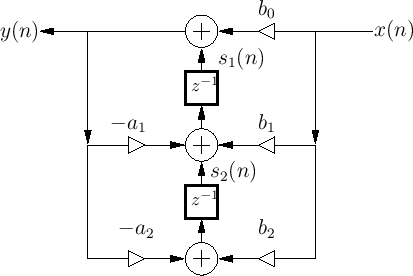
\includegraphics[scale=0.6]{photos/df2t.png}
 \caption{Direktna II transponirana realizacija filtra}
 \label{df2t}
\end{figure}

Složenost proračuna kod direktne II transponirane realizacije drugog reda (za bikvadratne sekcije) jest: 5 množenja, 4 dvoulazna zbrajanja i 2 memorijske lokacije. S obzirom da koristimo IIR butterworth filtar sa sedam koefijenata, imamo 2?? bikvadratne sekcije te tipe imamo sveukupno 10 množenja, 8 dvoulaznih zbrajanj te 4 memorijske lokacije za stanja. Ako usporedimo sa FIR relizacijom filtra i uzmemo u obzir 40 filtarskih koeficijenata da bi postigli jednake performanse kao i IIR filtar, imamo sveukupno: 40 množenja, 1 zbrajanje te nemamo memorijskih lokacija.


S obzirom da se radi o Cortex-M4 procesoru koji ima podršku za MAC i SIMD instrukcije koje su objašnjene u poglavlju \ref{SIMD}, procesno vrijeme se dvostruko ubrzava.

*Podatke o količini zbrajanja, množenja te količina potrebnih memorijskih lokacija se treba još jednom provjeriti te napraviti usporedbu s korištenjem FIR filtara*
\section{Vanjske komponente}
\subsection{MEMS mikrofon}
MEMS (eng. \textit{MicroElectrical-Mechanical System}) mikrofoni pogodni su za ugradbene računalne sustave zbog svog dobrog omjera signala prema šumu, male potrošnje energije, dolazi u vrlo malim pakiranjima te su odličnih temperaturnih karakteristika.

Ovakvi mikrofoni su uglavnom omnidirekcijski (primaju signale iz svih smjerova) te ih je moguće koristiti u raznim aplikacijama poput VoIP, u prijenosnim računalima, anti-theft sustavima i slično.

Postoje dvije izvedbe MEMS mikrofona, a to su analogna i digitalna verzija. U oba slučaja mikrofon se sastoji od fiksne i pomične membrane te se pomicanjem membrane tijekom akvizicije signala mjeri kapacitivnost između dviju membrana. Ono što u analognoj izvedbi dobijemo kao izlaz naponski, dok u digitalnoj izvedbi dobijemo PDM signal.

*Potrebno još proširiti poglavlje i dodatno pojasniti*

\begin{figure}[hbt!]
 \centering
 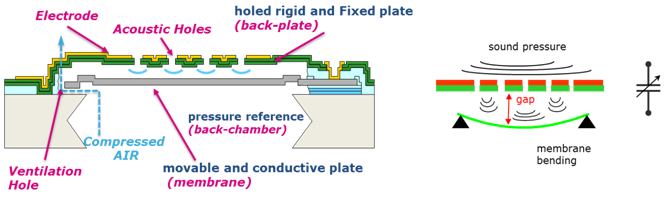
\includegraphics[scale=0.8]{photos/gradjamems.png}
 \caption{Tehnička izvedba MEMS mikrofona}
 \label{SIMD}
\end{figure}

\section{Komunikacija unutar ugradbenog računalnog sustava}
\section{Audio kodek}
Za potrebe akvizicije i obrade signala, koristi se STM-ov razvijeni kodek. Kodek definira potrebne protokole za komunikaciju sa mikrofonom, slanje signala na obradu te pomoću DMA reprodukciju signala na izlazu. Za potrebe razumijevanja aplikacije, razjasnit će se komunikacija mikrofon - procesor te procesor - izlaz.

\subsection{Komunikacija mikrofon - kodek}
Ova komunikacija je omogućena putem I2S protokola. I2S protokol podržava komunikaciju u slučaju prijenosa audio signala. Ovaj protokol spada pod SPI protokole (engl. \textit{serial peripheral interface}). Takvi protokoli definiraju komunikaciju uređaja sa perifernim komponentama, u ovom slučaju mikrofonom, te definiraju koji uređaj vodi komunikaciju (engl. \textit{master}) te koji sluša (engl. \textit{slave}).

Ono što je potrebno definirati jest koji uređaj vodi komunikaciju, a taj uređaj će davati \textit{slave-u} \textit{clock} koji određueje brzinu prijenosa podataka koji također moramo omogućiti u konfiguraciji. Zatim definiramo frekvenciju uzorkovanja koja će u našem slučaju biti 24 kHz. Naravno, da bi \textit{master} znao kojem uređaju šalje \textit{clock}, inicijaliziraju se i GPIO jedinice koje to omogućuju. Na taj način su uređaji usklađeni te mogu početi s komunikacijom.  

\subsection{Komunikacija kodek - izlaz}
Za potrebe komunikacije kodeka i izlaza bitan je protokol I2C.

I2C protokol je serijska vrsta komunikacije između \textit{mastera} i \textit{slave-a}. Koristi dvije linije komunikacije, jedna je za prijenos podataka (SDA) i jedna je za prijenos \textit{clocka}. 

*Proširiti*
\subsection{PDM filtar}
S obzirom da se koristi MEMS mikrofon koji daje digitalni izlaz u obliku PDM-a (engl.\textit{pulse density modulation}), takav izlaz je potrebno pretvoriti u informaciju koja se može čitati na izlazu, a to je zvuk u obliku PCM-a (engl. \textit{pulse code modulation})

STMicroelectronics su razvili PDM filtar koji vrši pretvorbu PDM-a u PCM. To radi na način da pomoću dva IIR filtra (niskopropusnog i visokopropusnog) te decimatora 1 bit PDM signala pretvori u PCM signal. 

Kako bi daljna obrada signala bila valjana, ključno je odrediti veličine ulaznog i izlaznog međuspremnika. Za ulazni buffer iznosi:

$input\_buffer = \frac{out\_freq* dec\_factor * inpu\_mic\_chn}{100*8}$

Za izlazni buffer iznosi:

$output\_buffer = \frac{out\_frequency* out\_mic\_chn}{1000} $

*dodati footnote za pdm i pcm*

\chapter{Napredna obrada digitalnog signala}
Prilikom implementacije grafičkog ekvilajzera, nije moguće koristiti kaskadnu ili paralelnu realizaciju filtra. Primjerice, ako imamo područje oko 600 Hz i 3000 Hz koje želimo naglasiti ili prigušiti, prilikom filtracije će si filtri međusobno poremetiti djelovanje te nećemo dobiti željena svojstva signala. U ovakvom slučaju se koriste filtarske banke.

\section{Izvedba filtarskih realizacija}\label{filtri}
U poglavlju \ref{chap:sluh} smo se upoznali s činjenicom da je raspon ljudskog slušnog područja od 20 Hz do 20000 Hz, no isto tako prilikom govora možemo primijetiti da se u tom rasponu kreće i frekvencijski spektar samog govora, što znači da prilikom govora osobe, pogotovo djeca koja imaju prirodno viši glas, mogu generirati frekvencije i iznad 10000 Hz (prilikom izgovora glasa C). 

Tako je potrebno generirati 18 pojasno propusnih filtara  čiji su parametri usklađeni s međunarodnim standardima i preporukama (ISO R 266, DIN 401 i ANSI S1.1-2004). Razlog odabira točno 18 pojaseva će biti razjašnjeno u jednom od sljedećih poglavlja.
 
Za realizaciju filtra moguć je odabir između optimalnog FIR filtra i Butterworth filtra. 

Butterworth filtar jest tip digitalnog filtra proizišao iz analogne realizacije istoimenog filtra od strane britanskog inženjera Stephena Butherwortha kojeg je predstavio u svom članku "On the Theory of Filter Amplifiers". Glavna značajka ovog tipa filtra jest to što je on maksimalno gladak. To znači da je jednako osjetljiv za svaku frekvenciju ovisno o području propuštanja. Također, za razliku od Cheby I/II i eliptičke izvedbe IIR filtra, Butterworth među ovim realizacijama jedini ima približno linearnu fazu što je nemoguće postići sa prethodno spomenutim filtrima.

Butterworth filtar predstavlja IIR tip filtra (eng. \textit{infinite impulse response}). Izlaz IIR filtra ovisi o svom ulazu te je impulsni odziv sljedeći:

\begin{equation}
\begin{aligned}
\sum_{l=0}^{N}a_{l}y[n-l] = \sum_{k=0}^{M}b_{k}x[n-k]
\end{equation}
\end{aligned}

gdje $N$ i $M$ predstavljaju broj uzoraka na ulazu i izlazu, slijedom.

Razlog zbog kojeg je u nekim slučajevima češće korišten IIR tip filtra jest zbog svojeg dobrog gušenja nepropusnog dijela sa vrlo malim brojem filtarskih koeficijenata, za razliku od FIR filtra. Zašto je ovaj faktor iznimno bitan jest zbog smanjenja vremena procesiranja signala. Na slici ... možemo vidjeti FIR i IIR realizacije filtara za isto pojasnopropusno područje. FIR filtar je realiziran s 50 koeficijenata, a IIR filtar sa 7 koeficijenata. 

*Dodati sliku*


S druge strane, postoji opcija realizacije sustava s optimalnim FIR filtrima. Ovaj filtar dizajnira se iterativnim Parks-McClellan algoritmom koji omogućuje minimiziranje maksimalne greške te korisniku dopušta da eksplicitno odredi širinu prijelaznog područja, razinu gušenja te razinu valovitosti u prijelaznom području. Iako u konačnici ovakav filtar za pristojna svojstva implementacije sustava za obradbu govora ima najčešće preko 40 koeficijenata, ono što je ključno kod njega jest linearna faza.

Također, koeficijenti filtra je potrebno pretvoriti u 16-bitne cjelobrojne koeficijente. Slika *Dodati sliku* prikazuje ponašanje izvornog filtra te 16-bitnu varijantu. Ono što se može uočiti je da filtar ne gubi svoju izvornu kvalitetu pri kvantizaciji koeficijenata tako da se mogu očekivati dobre performanse filtriranja te uštedu na vremenu pri filtriranju na mikrokontroleru. 

\section{Filtarske banke}
Filtarske banke jesu struktura koja na prethodno definirani broj pojasnih filtara šalje ulazni signal te nakon filtracije sve pojaseve zbraja te šalje na izlaz. Iako ovakva filtracija signala troši procesne resurse, za svaki filtar se može zasebno odrediti razina pojačanja/gušenja svakog pojasa. Na taj način ostali pojasevi ostaju netaknuti.

\section{S1.11 ANSI 2004}
U inačici S1.11 ANSI 2004 standarda definira se dizajn oktavno i frakcionalno oktavnih filtara. Ključna stvar kod definicije ovakvih filtara jest centralna frekvencija i razina gušenja filtra.

U ovom slučaju fokus će bit na implementaciju tercno-oktavnih filtarskih banka. Koa određivanja centralnih frekvencija koristi se formula:
\begin{equation}
\begin{aligned}
f_c = 2^\frac{x-3}{30}*f_m   [Hz]
\end{aligned}
\end{equation}

gdje je $x$ redni broj banke koju želimo dizajnirati, a kod $f_m$ se kao referentna vrijednost uzima 1000 Hz. Također, ovakvi filtri imaju već unaprijed definiran pojas propuštanja, koji ovisi centralnoj frekvenciji filtra, a izračuna se na sljedeći način:

\begin{equation}
\begin{aligned}
f_d = \frac{f_c}{2^\frac{1}{6}}
\end{aligned}
\end{equation}
\begin{equation}
\begin{aligned}
f_g = f_c \cdot 2^\frac{1}{6}
\end{aligned}
\end{equation}

primjerice, u slučaju da imamo centralnu frekvenciju 200 Hz, gornja granična frekvencija iznosi 224,49 Hz, a donja 178.18 Hz. Širina tog pojasa iznosi svega 46.31 Hz, uzevši u obzir našu frekvenciju uzorkovanja, to je jako usko područje te bi bilo potrebno više koeficijenata za njegovu realizaciju.

Nakon određivanja centralnih frekvencija te pojasa propuštanja, potrebno je odrediti tip filtra koji će se koristiti te jedna od vrsta te vrste filtra \citep{ansi2004}.

Između već poznata dva tipa filtra (FIR i IIR), najčešći odabir za FIR filtar jest optimalni FIR filtar dizajniran Parks-McLellan metodom i Butterworth filtar opisani u poglavlju \ref{filtri}.

\chapter{Algoritam višepojasnog filtriranja}
Uzimajući u obzir da se obradba govora izvršava na ugradbenom sustavu, treba se imati na umu ograničenja procesiranja signala, tako da je potrebno maksimalno optimizirati sustav za rad u stvarnom vremenu. Tako u članku vezano za razvoj algoritma za obradbu signala za slušne aparate imamo ponuđeno rješenje koje itekako može koristiti u našem slučaju.

Srž sustava za filtiriranje će se bazirati na decimiranim slogovima

*Proširiti*
\citep{fbdha}



\chapter{Analiza performansi sustava}
\section{Obrada govora u MATLAB-u}
U MATLAB-u je razvijeno grafičko sučelje koje omogućuje odabir optimala, odabir pojačanja pojasa glasa te prekid filtriranja kako bi se mogao usporediti izlazni signal.

Filtriranje je implementirano pomoću Butterwortovog filtra s kvantiziranim 16-bitnim koeficijentima.

*Proširiti*

\begin{lstlisting} 
while true
    audio = record(fileReader);
    j=1;
     for i=1:20
          if(i==offset(j))
             a  = sosfilt(C{1,i},audio); 
             if(j<4)
                 j = j+1;
             end
          else
             a  = sosfilt(C{1,i},audio);
          end
          out = out + a;

     end
    i=1;

    
    step(deviceWriter, out);
    out=0;
    a=0;

 end
\end{lstlisting}

Gornja implementacija filtriranja radi to na sljedeći način:

Za svaku optimalu su definirani pojasevi koji se naglašavaju za rehabilitaciju poremećaja kod izgovora pojedinih glasova. Pojasevi su definirani u strukturi prema odmaku od prvog pojasa. Na taj način se samo za te pojaseve definira pojačanje te ostali pojasevi ostanu netaknuti.


Pomoću AudioProcessingToolboxa omogućeno je snimanje i reproduciranje u stvarnom vremenu. Postoji mogućnost odabira uređaja putem kojeg se vrši akvizicija i reprodukcija zvuka, što je u našem slučaju vanjska zvučna kartica marke Yamaha Steinberg.

*Proširiti*

\section{Grafičko sučelje za obradu govora}

Također, u MATLAB-u je razvijeno grafičko sučelje za obradu govora temeljenu na optimalama. Ovakav program omogućuje inicijalizaciju filtarskih pojaseva, reprodukciju zvuka bez i s obradom. Moguć je odabir optimala od svih glasova u hrvatskom jeziku te pojačanje koje se vrši na optimalama.

\begin{figure}[hbt!]
\label{gui}
 \centering
 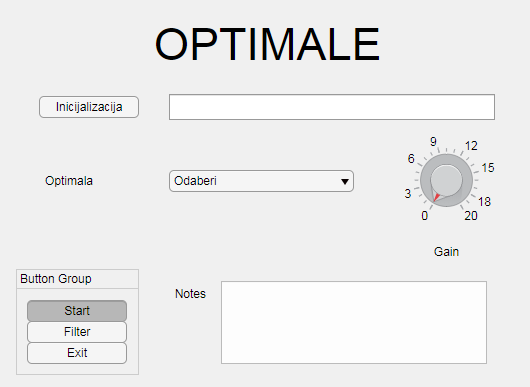
\includegraphics[scale=0.5]{photos/gui.png}
 \caption{Izgled grafičkog sučelja u MATLAB-u}
\end{figure}

Na slici \ref{gui} uočavamo dio za inicijalizaciju; ono omogućuje dizajn filtara koji koristimo za ove potrebe, a to su tercno-oktavni filtri. Sljedeće se pritiskom gumba \textit{Start} pokreće reprodukcija zvuka u stvarnom vremena s određenom latencijom koja u našem slučaju nije zanemariva. \textit{Filter} gumb pokreće filtraciju pomoću optimala. Prethodno prije pokretanja obrade se treba odabrati optimala te pojačanje (u slučaju ne odabiranja pojačanja, na izlazu će biti isti zvuk kao i na ulazu). 

\section{Ograničenja sustava}
Tijekom razvoja sustava moguće je doći do određenih komplikacija koje usporavaju ili onemogućavaju razvoj sustava. U ovom poglavlju će se tako navesti neke mane razvojnog sustava STM32F4-Discovery koji je u ovom slučaju trebao služiti za obradbu govora te će se problemi slijedno opisati od same akvizicije signala preko obradbe do reprodukcije.

\subsection{Mikrofon}
Tako prvi na redu dolazi mikrofon koji je integrirn na samom mikrokontroleru, to jest nije uzeta nikakva vanjska komponenta za mikrofon. Integrirani mikrofon je model MP34DT06J, digitalni MEMS omnidirekcijski mikrofon. Ovaj mikrofon ima široku upotrebu, od raspoznavanja govora do mikrofona u prijenosnim računalima. Iako se naoko čini da će ovakav mikrofon bez dodatnih problema vršiti akviziciju signala, s obzirom na mogućnosti implementacije unutar samog mikrokontrolera, s odabirom frekvencije uzorkovanja veće od 16 kHz dobijemo većinski šum, a samim pogledom na \textit{datasheet} vidimo da je uzrok tog problema frekvencijska karakteristika samog mikrofona, točnije mi ne znamo ponašanje mikrofona kod frekvencija većih od 10 kHz \citep{mic}. No, pregledom ponude MEMS mikrofona različitih proizvođača, ne ostavlja puno izbora za odabir komponente koja će se ponašati približno kvalitetno kao i komercijalni profesionalni mikrofon koji pokriva cijelo slušno područje čovjeka.

\subsection{Jezgra sustava za obradbu govora}
Kod analize same obradbe govora nailazimo na dva problema: mogućnost procesiranja 18 pojaseva signala te sama filtracija signala. Što se tiče procesiranja signala, u sluč (naknadno će se opisati)

Filtracijom signala s već ponuđenim funkcijama unutar CMSIS-DSP biblioteke nailazimo na jedan dodatan problem. Iako Cortex-M4 ima mogućnost rada sa \textit{floating point} podacima, to nikako ne bi bilo dobro koristiti s obzirom da imamo ograničenu moć procesiranja, tako radimo s cjelobrojnim podacima; s ulaza nam dolaze 16-bitni podaci, a filtri su nam idealno 16-bitni. No, ukoliko su dizajnirani Butterworth filtri u MATLAB-u, ne dobiju se koeficijenti u rasponu -1 do 1 nad kojima je potrebno primijeniti frakcionalnu aritmetiku, već dobijemo brojeve koji nam nadilaze pa čak i 6 što znači da na puno kompleksniji način, pa čak dolazimo do nemogućnosti pakiranja koeficijente u 16-bitne varijable. To nam dodatno komplicira implementaciju sustava jer DSP funkcije nude implementaciju isključivo ako su podaci s mikrofona i koeficijenti filtra jednake veličine. S druge strane, moguć jest odabir FIR filtra, ali u tom slučaju riskiramo porast koeficijenata najčešće 10 puta, kako bi imali približno jednake performanse filtra.

\subsection{Kašnjenje}
Ovaj problem se javlja i unutar MATLAB aplikacije i unutar mikrokontrolera. S obzirom da je ovaj razvijeni uređaj namijenjen za rehabilitacijske svrhe izgovora određenih glasova, tako govornik ne smije biti u mogućnosti percipirati kašnjenje zvuka jer time uređaj gubi svrhu. MATLAB tu ne nudi rješenje, sama inicijalizacija APIja koji komunicira sa zvučnom karticom traje preko 200 ms, a akvizicija i reprodukcija zvuka zajedno isto 200 ms. Naravno, kašnjenje je usko povezano sa veličinom ulaznog međuspremnika, no, odabirom međuspremnika veličine manje od 1024 uzoraka, signal se jednostavno ne stigne obraditi i poslati na izlaz. Tako je korisnik primoran postaviti međuspremnik sa 2048 uzorka te riskirati kašnjenje signala.

Kod samog STM-a, moguć problem kašnjenja jest što razvojni sustav jednostavno nije prilagođen za visokokvalitetnu obradbu signala. Tako samo očitavanje signala sa frekvencijom većom od 16 kHz uzima preveliku količinu vremena za očitavanje. U ovom slučaju svakako je poželjno napraviti kompromis, a to je uzimanje frekvencije očitavanja od 24 kHz koja onda pokriva područje do 12 kHz. Nije idealno, ali se smanjuje vrijeme procesiranja i očitavanja signala te se pokriva većina područja koje ljudsko uho čuje. Također, pozitivna stvar kod implementacije sustava na mikrokontroleru što je međuspremnik od 512 uzoraka dostatan za normalnu obradbu i reprodukciju signala.
\chapter{Zaključak}
Zaključak.

\bibliography{literatura}
\bibliographystyle{fer}

\begin{sazetak}
Sažetak na hrvatskom jeziku.

\kljucnerijeci{digitalna obradba signala, digitalna obradba govora, ugradbeni računalni sustavi, filtarske banke, tercno-oktavni filtri, STM32F4-Discovery, MATLAB, ARM Cortex-M4 grafički ekvilajzer, rehabilitacija govora, optimale, verbotonalna metoda}
\end{sazetak}

% TODO: Navedite naslov na engleskom jeziku.
\engtitle{Embedded System for Real Time Speech Signal Processing and Analysis}
\begin{abstract}
Abstract.

\keywords{digital signal processing, speech processing, embedded systems, filter banks, third-octave filters, STM32F4-Discovery, MATLAB, ARM Cortex-M4, graphic equalizer, speech rehabilitation, optimals, verbotonal method}
\end{abstract}

\end{document}
